\documentclass{article}
\usepackage{xeCJK}
\setCJKmainfont{SimSun}
\usepackage{multirow}
\usepackage{graphicx}
\usepackage{booktabs} % for better table formatting
\usepackage{geometry} % for adjusting page layout
\usepackage{enumitem} % for customizing lists
\usepackage{hyperref} % for clickable links and references
\usepackage{subcaption}

% Set the margins
\geometry{
 a4paper,
 left=20mm,
 right=20mm,
 top=25mm,
 bottom=25mm
}

\title{软件测试}
\author{高丁超} % add author name if needed
\date{} % remove date or add specific date

\begin{document}
\maketitle
\linespread{1.5}
\section{Python for Image Computation}
\begin{itemize}[leftmargin=*]
    \item 软件的工作目标: 
    \begin{itemize}
        \item 输入电路与系统初始状态,输出下一步的系统状态。
    \end{itemize}
    \item 运行环境:
    \begin{itemize}
        \item Python >= 3.9.0
        \item Numpy >= 1.20.0
        \item Qiskit >= 0.25.0
        \item Graphviz >= 0.20.0
    \end{itemize} 
    \item 适应的工作对象:
    \begin{itemize}
        \item 复杂线路如Grover,QRW不超过二十比特。
        \item 简单线路如GHZ,不超过二百比特。
    \end{itemize}
    \item 测试样例:
    \begin{itemize}
        \item Grover
        \item QFT
        \item BV
        \item GHZ
        \item QRW
    \end{itemize}
    \item 自我测试实验报告:
    \begin{itemize}
        \item  \linespread{1.5}图\ref{fig:grover-compare}表示了对Grover搜索算法运行不同image computation算法的资源对比。图\ref{fig:QFT-compare}表示了对quantum Fourier transform(QFT)算法运行不同image computation算法的资源对比。图\ref{fig:BV-compare}表示了对Bernstein–Vazirani(BV)算法运行不同image computation算法的资源对比。图\ref{fig:GHZ-compare}表示了对Greenberger–Horne–Zeilinger (GHZ)状态制备电路运行不同image computation算法的资源对比。图\ref{fig:QRW-compare}表示了对在$2^n$ 环上的quantum random walk (QRW)算法运行不同image computation算法的资源对比。
        \begin{figure}[!htbp]
            \centering
            \begin{subfigure}[b]{.4\textwidth}
                \centering
                \includegraphics[height=4cm]{Img/alg_Grover_time.pdf}
                \caption{对Grover 算法应用不同电路拆分技术的时间对比}
                \label{fig:grover-time}
            \end{subfigure}
            \qquad
            \begin{subfigure}[b]{.4\textwidth}
                \centering
                \includegraphics[height=4cm]{Img/alg_Grover_node.pdf}
                \caption{对Grover 算法应用不同电路拆分技术的最大节点对比}
                \label{fig:grover-node}
            \end{subfigure}
            
            \caption{对Grover算法运行image computation时不同电路拆分技术的资源对比}
            \label{fig:grover-compare}
        \end{figure}
        \begin{figure}[!htbp]
            \centering
            \begin{subfigure}[b]{.4\textwidth}
                \centering
                \includegraphics[height=4cm]{Img/alg_QFT_time.pdf}
                \caption{对QFT 算法应用不同电路拆分技术的时间对比}
                \label{fig:QFT-time}
            \end{subfigure}
            \qquad
            \begin{subfigure}[b]{.4\textwidth}
                \centering
                \includegraphics[height=4cm]{Img/alg_QFT_node.pdf}
                \caption{对QFT 算法应用不同电路拆分技术的最大节点对比}
                \label{fig:QFT-node}
            \end{subfigure}
            \caption{对QFT算法运行image computation时不同电路拆分技术的资源对比}
            \label{fig:QFT-compare}
        \end{figure}
        \begin{figure}[!htbp]
            \centering
            \begin{subfigure}[b]{.4\textwidth}
                \centering
                \includegraphics[height=4cm]{Img/alg_BV_time.pdf}
                \caption{对BV 算法应用不同电路拆分技术的时间对比}
                \label{fig:BV-time}
            \end{subfigure}
            \qquad
            \begin{subfigure}[b]{.4\textwidth}
                \centering
                \includegraphics[height=4cm]{Img/alg_BV_node.pdf}
                \caption{对BV 算法应用不同电路拆分技术的最大节点对比}
                \label{fig:BV-node}
            \end{subfigure}
            \caption{对BV算法运行image computation时不同电路拆分技术的资源对比}
            \label{fig:BV-compare}
        \end{figure}
        \begin{figure}[!htbp]
            \centering
            \begin{subfigure}[b]{.4\textwidth}
                \centering
                \includegraphics[height=4cm]{Img/alg_GHZ_time.pdf}
                \caption{对GHZ 算法应用不同电路拆分技术的时间对比}
                \label{fig:GHZ-time}
            \end{subfigure}
            \qquad
            \begin{subfigure}[b]{.4\textwidth}
                \centering
                \includegraphics[height=4cm]{Img/alg_GHZ_node.pdf}
                \caption{对GHZ 算法应用不同电路拆分技术的最大节点对比}
                \label{fig:GHZ-node}
            \end{subfigure}
            \caption{对GHZ算法运行image computation时不同电路拆分技术的资源对比}
            \label{fig:GHZ-compare}
        \end{figure}
        \begin{figure}[!htbp]
            \centering
            \begin{subfigure}[b]{.4\textwidth}
                \centering
                \includegraphics[height=4cm]{Img/alg_QRW_time.pdf}
                \caption{对QRW 算法应用不同电路拆分技术的时间对比}
                \label{fig:QRW-time}
            \end{subfigure}
            \qquad
            \begin{subfigure}[b]{.4\textwidth}
                \centering
                \includegraphics[height=4cm]{Img/alg_QRW_node.pdf}
                \caption{对QRW 算法应用不同电路拆分技术的最大节点对比}
                \label{fig:QRW-node}
            \end{subfigure}
            \caption{对QRW算法运行image computation时不同电路拆分技术的资源对比}
            \label{fig:QRW-compare}
        \end{figure}
        \item 表\ref{table:time}给出了在不同电路拆分技术下具体的各类算法的计算时间,单位为秒,max node表示计算过程中TDD的节点最大个数,- 表示超时。其中addition 和contraction表示不同的电路拆分技术。
    \begin{table}[!htbp]
        \centering
        \scalebox{0.5}{
            \begin{tabular}{llllllllll}
                \hline
                \multirow{2}{*}{Benchmark} &  & \multicolumn{2}{c}{basic} &  & \multicolumn{2}{c}{addition} &  & \multicolumn{2}{c}{contraction} \\ \cline{3-4} \cline{6-7} \cline{9-10} 
                                           &  & time        & max \#node       &  & time          & max \#node        &  & time           & max \#node          \\ \hline
                Grover\_15 &   & 19.33  & 15785     &   & 17.35      & 15099  & & 1.61 & 597  \\
                Grover\_18 &   & 76.47  & 61694     &   & 66.02      & 60332  & & 2.41 & 516  \\
                Grover\_20 &   & 294.65 & 243946    &   & 259.87     & 241240 & & 4.39  & 1036 \\ 
                Grover\_40 &   & -      &           &   & -          &        & & 2953.57 & 851973 \\
                \hline
                QFT\_15     &  & 34.64   & 65536   &  & 18.88  & 32770   &  & 0.08 & 63  \\
                QFT\_18     &  & 282.12  & 524288  &  & 148.13 & 262146 &   & 0.10  & 31  \\
                QFT\_20     &  & 1199.21 & 2097152 &  & 655.19 & 1048578 &  & 0.12 & 63  \\
                QFT\_30     &  & -       &         &  & -      &        &  & 0.29 & 31  \\
                QFT\_50     &  & -       &         &  & -      &        &  & 1.02 & 51  \\
                QFT\_100    &  & -       &         &  & -      &        &  & 7.14 & 101 \\
                \hline
                BV\_100     &  & 7.36    & 596     &  & 7.43      & 596     &  & 0.41           & 102 \\
                BV\_200     &  & 31.57   & 1196    &  & 30.03     & 1196    &  & 1.70           & 202 \\
                BV\_300     &  & 75.66   & 1796    &  & 75.56     & 1796    &  & 4.28           & 302 \\
                BV\_400     &  & 146.47  & 2396    &  & 145.40    & 2396    &  & 9.18           & 402 \\
                BV\_500     &  & 244.15  & 2996    &  & 223.90    & 2996    &  & 16.31          & 502 \\
                \hline
                GHZ\_100    &  & 0.38    & 595     &  & 0.13      & 301    &  & 0.18           & 200 \\%& 0.03    
                GHZ\_200    &  & 0.72    & 1195    &  & 0.37      & 601    &  & 0.48           & 400 \\%& 0.12     
                GHZ\_300    &  & 1.29    & 1795    &  & 0.62      & 901    &  & 0.80           & 600 \\%& 0.24     
                GHZ\_400    &  & 2.03    & 2395    &  & 1.00      & 1201    &  & 1.26           & 800 \\%& 0.42     
                GHZ\_500    &  & 2.96    & 2995    &  & 1.45      & 1501    &  & 1.72           & 1000\\%& 0.62     
                \hline
                QRW\_15     &  & 36.86   & 13122     &  & 24.59     & 10882     & & 7.16  & 222 \\
                QRW\_18     &  & 139.76  & 90538     &  & 84.69     & 37064     & & 11.23 & 226 \\
                QRW\_20     &  & 341.05  & 265614    &  & 218.29    & 107714    & & 14.31 & 404 \\
                QRW\_30     &   &-       &          &  &-          &          & & 36.82 & 404 \\
                QRW\_50     &   &-       &          &  &-          &          & & 118.08 & 404 \\
                QRW\_100    &   &-       &          &  &-          &          & & 692.08 & 436 \\
                \hline
            \end{tabular}
        }
        \caption{对不同测试实验应用image computation}
        \label{table:time}
    \end{table}
    \end{itemize}
    
\end{itemize}
\newpage
\section{C++ for TDD}
\begin{itemize}[leftmargin=*]
    \item 软件的工作目标: 
    \begin{itemize}
        \item 输入电路,输出电路的TDD表示。
    \end{itemize}
    \item 运行环境: 
    \begin{itemize}
        \item C++ Standard 17
        \item CMake >= 3.20.0
        \item XTL >= 0.7.5
        \item XTENSOR >= 0.24.0
        \item Graphviz >= 2.43.0
        \item XTENSOR-Python >= 0.26.0
        \item Pybind11 >= 2.12.0
        \item Numpy >= 1.20.0
    \end{itemize} 
    \item 适应的工作对象:
    \begin{itemize}
        \item 小型电路
    \end{itemize}
    \item 测试样例:
    \begin{itemize}
        \item 基础门,如CNOT, H, S, Swap
        \item 随机生成的小规模电路
    \end{itemize}
    \item 自我测试实验报告:
    \begin{itemize}
        \item 所有基础门正确转化为TDD表示。
        \item 支持任意维度张量,例如对双比特CNOT门,既可以按图\ref{fig:cnot-4}中的张量维度为4,
        即按照索引为$q_1,q_0$进行表示。也可以按图\ref{fig:cnot-2}中的张量维度为4,
        即按照索引为$q_3,q_2,q_1,q_0$进行表示。这样的设计大大提高了TDD的表示能力,为更复杂系统的验证提供了基础。
        \begin{figure}[!htbp]
            \centering
            \begin{subfigure}[b]{.4\textwidth}
                \centering
                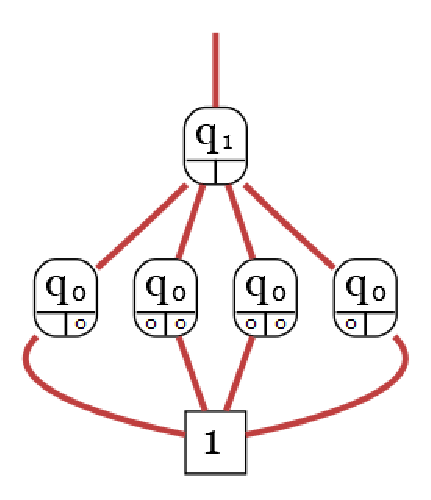
\includegraphics[height = 6cm]{Img/cnot.eps}
                \caption{张量维度为4的CNOT门的TDD表示}
                \label{fig:cnot-4}
            \end{subfigure}
            \begin{subfigure}[b]{.4\textwidth}
                \centering
                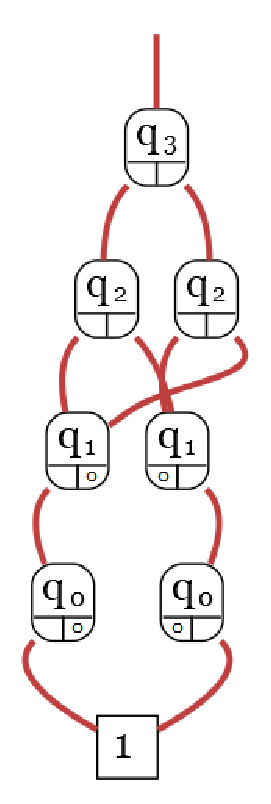
\includegraphics[height=6cm]{Img/cx.eps}
                \caption{张量维度为2的CNOT门的TDD表示}
                \label{fig:cnot-2}
            \end{subfigure}
            \caption{C语言版的TDD支持任意维度的例子}
            \label{fig-cnot}
        \end{figure}
    \end{itemize}
\end{itemize}
\end{document}